\documentclass[a4paper]{article}

\usepackage[T2A]{fontenc}
\usepackage[utf8]{inputenc}
\usepackage[russian]{babel}
\usepackage{graphicx}
\usepackage{float}
\usepackage{mathtools}
\usepackage{wrapfig}
\usepackage{amsfonts, amssymb, amsmath, latexsym}
\usepackage{nicefrac}
\usepackage{hhline}
\usepackage{multirow}
\usepackage[colorlinks=true,linkcolor=black,citecolor=blue]{hyperref}       % hyperlinks
\usepackage{nicefrac}       % compact symbols for 1/2, etc.
\usepackage{nameref}
\usepackage{booktabs}       % professional-quality tables
\usepackage{algorithm}
\usepackage{algpseudocode}
\usepackage{xcolor, colortbl}
\usepackage{etoolbox}

% \graphicspath{ {./} }

\usepackage[verbose=true,letterpaper]{geometry}

\newgeometry{
    textheight=25cm,
    textwidth=18cm,
    top=2.5cm,
    headheight=12pt,
    headsep=10pt,
    footskip=1cm,
    marginparwidth=15pt
}

%\usepackage{showframe} 

\usepackage{epigraph}
\usepackage{amsmath,amsfonts,amssymb,amsthm,mathtools, mathrsfs}
\usepackage{amsthm}

\title{Работа 5.8.1 \\ Тепловое излучение}
\author{Колесников Иван, Шарапов Денис, Б05-004}
\date{}

\usepackage{fancyhdr}
\pagestyle{fancy}
\fancyhf{}
\rhead{Работа 5.8.1}
\lhead{}
\cfoot{\thepage}
\usepackage{subcaption}
\usepackage[font={small}]{caption}

\begin{document}

    \maketitle
    \tableofcontents
    \newpage
    
\section{Аннотация}

\noindent\textbf{Цель работы:} при помощи модели абсолютно чёрного тела провести измерения температуры
оптическим пирометром с исчезающей нитью и термопарой; исследовать излучение накалённых тел с различной испускательной способностью; определить постоянныe Планка и Стефана-Больцмана. \smallskip
 
\noindent \textbf{В работе используются:} оптический пирометр, модель абсолютно чёрного тела, образцы колец, вольфрамовая
лампа, неоновая лампа, блок питания, цифровые вольтметры.

\section{Теоретические сведения}

Для измерения температуры разогретых тел, удалённых от наблюдателя, применяют методы оптической пирометрии, основанные на использовании зависимости испускательной способности исследуемого тела от температуры. Различают три температуры, функционально связанные с истинной термодинамической температурой и излучательной способностью тела: радиационную, цветовую и яркостную. \medskip

\noindent В работе измеряется яркостная температура. Яркостная температура - это температура абсолютно чёрного тела, при которой его спектральная испускательная способность равна спектральной испускательной способности исследуемого тела при той же длине волны. Измерение яркостной температуры раскалённого тела производится при помощи оптического пирометра с исчезающей нитью, основанного на визуальном сравнении яркости раскалённой нити с яркостью изображения исследуемого тела. \medskip


\noindent Яркостная температура тела всегда ниже его термодинамической температуры. Это связано с тем, что любое нечёрное тело излучает меньше, чем АЧТ при той же температуре. Зависимость между яркостной и термодинамической температурами
вольфрама приведена на рис. \ref*{fig:graph1}

\begin{figure}[ht!]
    \centering
    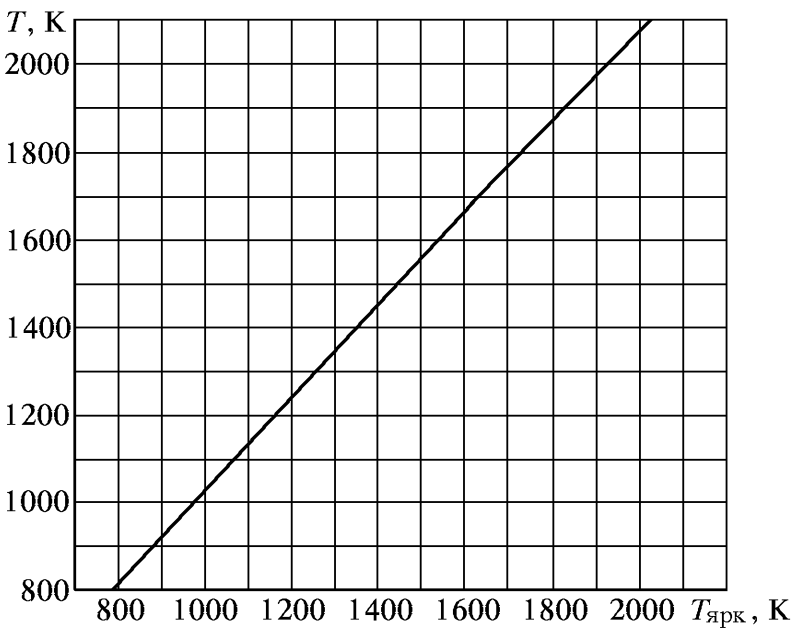
\includegraphics[width = 0.4\textwidth]{image/pic1.png}
    \caption{График зависимости $T = f(T_{\text{ярк}})$ для вольфрама}
    \label{fig:graph1}
\end{figure}

\noindent По результатам измерений мощности излучения вольфрамовой нити можно судить о справедливости закона Стефана-Больцмана. Если бы нить излучала как АЧТ, то баланс потребляемой и излучаемой энергии определялся бы соотношением
$$W = \sigma S (T^4 - T_0^4),$$
где $W$ --- потребляемая нитью электрическая мощность, $S$ --- площадь излучающей поверхности нити, $T$ --- температура нити, $T_0$ --- температура окружающей среды. Однако вольфрамовая нить излучает как серое тело, и излучение её ослаблено по сравнению с АЧТ в $\varepsilon_{T}$ раз для любой волны при данной температуре тела $T$. Тогда, предположив, что
нить излучает как серое тело и с учётом того, $T_0 \ll T$, получим 
$$W = \varepsilon_{T}S \sigma T^4.$$

\section{Экспериментальная установка}

Экспериментальная установка представлена на рис. \ref*{fig:schema}. Исследуемые в работе образцы: 
\begin{enumerate}
    \item модель абсолютно чёрного тела - керамическая трубка, закрытая с одного конца и окружённая для теплоизоляции внешним кожухом. Температура в трубке измеряется с помощью термопары хромель-алюмель;
    \item керамическая трубка с набором колец из различных материалов, нагреваемая изнутри нихромовой спиралью. Материалы колец имеют различную излучательную способность;
    \item вольфрамовая нить электрической лампочки.
\end{enumerate}

\begin{figure}[ht!]
    \centering
    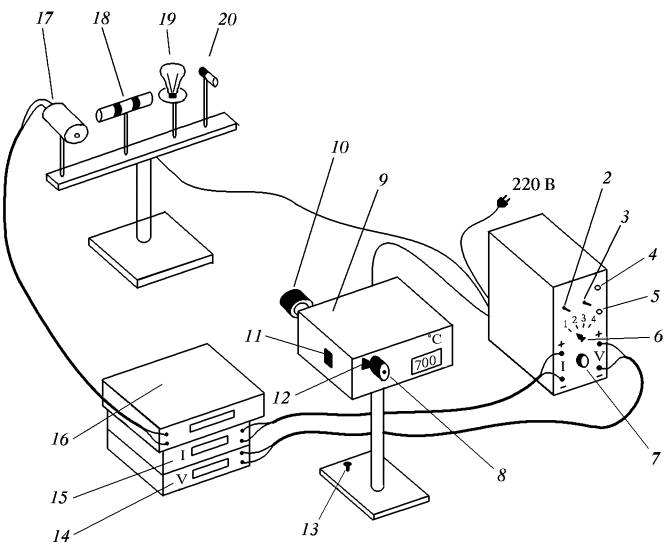
\includegraphics[width = 0.6\textwidth]{image/schema.png}
    \caption{Схема экспериментальной установки: 1 -- блок питания; 2 -- тумблер включения питания образцов;
    3 -- тумблер нагрева нити пирометра; 4 -- кнопка "Нагрев нити"; 5 -- кнопка "охлаждение нити"; 6 -- тумблер
    переключения образцов; 7 -- регулятор мощности нагрева образцов; 8 -- окуляр пирометра; 9 -- корпус
    пирометра; 10 -- объектив пирометра; 11 -- переключение диапазонов; 12 -- ручка смещения красного
    светофильтра; 13 -- регулировочный винт; 14 -- вольтметр~(напряжение на лампе накаливания); 15 --
    амперметр (ток через образцы); 16 -- вольтметр в цепи термопары; 17 -- модель АЧТ; 18 -- трубка с
    кольцами из материалов с различной излучательной способностью; 19 -- лампа накаливания; 20 --
    неоновая лампочка
    }
    \label{fig:schema}
\end{figure}


\section{Результаты измерений и обработка данных}

\subsection{Изучение работы оптического пирометра}

Изменяя ток через нить пирометра, добьёмся исчезновения нити на фоне изображения раскалённой поверхности дна АЧТ. Проверим корректность измерений: температура на пирометре не должна сильно отличаться от температуры АЧТ, измеренной термопарой. Результаты измерений занесём в таблицу \ref*{table:diff1} (постоянная термопары~$41 \;\; \text{мкВ}/^\circ C$).

\begin{table}[!ht]
    \centering
    \begin{tabular}{|c|c|c|c|c|}
    \hline
    $T_{\text{пир}}$, $^\circ C$ & $944$   & $961$   & $963$   & $956$   \\ \hline
    $T_{\text{АЧТ}}$, $^\circ C$ & $916$   & $925$   & $928$   & $930$   \\ \hline
    $U$, мВ                      & $37,54$ & $37,91$ & $38,04$ & $38,12$ \\ \hline
    $\Delta$, \%                 & $3,01$  & $3,78$  & $3,65$  & $2,75$  \\ \hline
    \end{tabular}
    \caption{Сравнение температуры нити пирометра и температуры АЧТ, где $\Delta$ -- разность значений температур, выраженная в процентах}
    \label{table:diff1}
    \end{table}

\noindent Разность температур не превышает $5\%$.

\subsection{Измерение яркостной температуры тел}

Измерим яркостную температуру нагретой керамической трубки и двух колец из разных материалов. Результаты измерения приведены в таблице \ref*{table:diff2}.

\begin{table}[!ht]
    \centering
    \begin{tabular}{|c|c|c|}
    \hline
    Керамическая трубка, $^\circ C$ & Кольцо 1, $^\circ C$ & Кольцо 2, $^\circ C$ \\ \hline
    $750 \div 850$                 & $\approx 750$        & $< 750$              \\ \hline
    \end{tabular}
    \caption{Измерение яркостной температуры при исследовании второго образца}
    \label{table:diff2}
\end{table}

\noindent Разность яркостных температур разных материалов при одинаковой термодинамической температуре объясняется разным  cпектральным коэффициентом поглощения.

\subsection{Проверка закона Стефана-Больцмана}

Постепенно увеличивая накал нити лампы, с $900 \; ^\circ C$ до $1900 \; ^\circ C$, будем измерять пирометром яркостную температуру нити, а также значение силы тока и напряжения на ней. По рис. \ref{fig:graph1}, используя линейную аппроксимацию, определим термодинамическую температуру нити. Результаты измерений представлены в таблице~\ref*{table:res1}.

\begin{table}[!ht]
    \centering
    \begin{tabular}{|c|c|c|c|c|}
    \hline
    $I$, мА & $U$, В  & $T_{\text{ярк}}$, $^\circ C$ & $T$, $^\circ C$ & $W$, мВт \\ \hline
    $0,64$  & $19,2$  & $900$                        & $920$           & $12,29$  \\ \hline
    $0,74$  & $27,3$  & $1000$                       & $1030$          & $20,20$  \\ \hline
    $0,75$  & $28,3$  & $1100$                       & $1140$          & $21,23$  \\ \hline
    $0,83$  & $34,7$  & $1200$                       & $1250$          & $28,80$  \\ \hline
    $0,89$  & $40,7$  & $1300$                       & $1350$          & $36,22$  \\ \hline
    $0,99$  & $49,6$  & $1400$                       & $1450$          & $49,10$  \\ \hline
    $1,12$  & $62,7$  & $1500$                       & $1550$          & $70,22$  \\ \hline
    $1,23$  & $75,3$  & $1600$                       & $1660$          & $92,62$  \\ \hline
    $1,33$  & $86,8$  & $1700$                       & $1770$          & $115,44$ \\ \hline
    $1,42$  & $97,7$  & $1800$                       & $1880$          & $138,73$ \\ \hline
    $1,56$  & $114,8$ & $1900$                       & $1980$          & $179,09$ \\ \hline
    \end{tabular}
    \caption{Зависимость мощности, выделяемой на лампе, от температуры нити накала ($S = 0,36 \; \text{см}^2$)}
    \label{table:res1}
    \end{table}

    \begin{figure}[ht!]
        \centering
        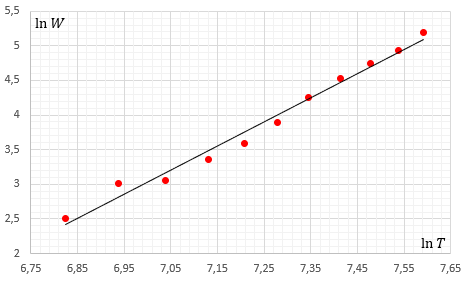
\includegraphics[width = 0.6\textwidth]{image/graph2.png}
        \caption{Зависимость мощности лампы от её термодинамической температуры, логарифмический масштаб}
        \label{fig:graph2}
    \end{figure}

\noindent Теоретическое значение показателя степени температуры в законе Стефана-Больцмана равно 4. Экспериментальное значение наклона кривой составляет $\approx 3,521 \pm 0,136$.

\begin{enumerate}
    \item Определим постоянную Стефана-Больцмана, используя значение термодинамической температуры $1980 \; ^\circ C$ (табличное значение) и соответствующую мощность. С помощью линейной аппроксимации получаем 
    $$\sigma_1 = (0,131 \pm 0,012) \cdot 10^{-12} \;\; \text{Вт} / (\text{см}^2\cdot\text{К}^4).$$

    \item Определим постоянную Стефана-Больцмана, используя построенный график \ref*{fig:graph2}:
    $$\sigma_2 = (5,614 \pm 0,008) \cdot 10^{-12} \;\; \text{Вт} / (\text{см}^2\cdot\text{К}^4).$$

    \item Теоретическое значение постоянной Больцмана: $$\sigma_{th} = 5,67 \cdot 10^{-12}\;\; \text{Вт} / (\text{см}^2\cdot\text{К}^4).$$
\end{enumerate}

Оценим постоянную Планка:
$$h = \left( \frac{2 \pi^5 k^4}{15 c^2 \sigma} \right)^{1/3} \approx 10^{-27} \;\; \text{эрг}\cdot\text{с}.$$

\subsection*{Измерение яркостной температуры неоновой лампочки}

Термодинамическая температура неоновой лампочки примерно равна комнатной температуре, и не соответствует её яркостной температуре $(\approx 850 \; ^\circ C)$. Это происходит засчёт того, неоновая лампочка не является моделью АЧТ, и её излучение носит совершенно другую природу (переход электронов между энергетическими уровнями).

\section{Вывод}

\noindent В ходе работы было изучено тепловое излучение модели абсолютно чёрного тела и моделей серых тел --- колец из различных материалов и вольфрамовой нити. Проверили выполнение закона Стефана-Больцмана на практике: скорее всего, этот закон не подтвердился из-за разности показаний пирометра и реальной термодинамической температуры тела. \medskip

\noindent Также наблюдали, что из-за различных коэффициентов спектрального поглощения материалов яркостная температура тел с одинаковой термодинамической температурой может не совпадать. \medskip

\noindent По результатам измерений была оценена постоянная Стефана-Больцмана двумя способами: непосредственно используя формулу и используя график зависимости $W(t)$ в логарифмическом масштабе. Второй способ оказался более точным. \medskip

\noindent В работе с помощью пирометра была определена яркостная температура неоновой лампочки, которая не является моделью АЧТ. Эта яркостная температура не совпадает с термодинамической. 

\end{document}
